\documentclass[10pt]{article}
\advance\hoffset by -0.7 truein\relax


\usepackage{graphicx}
%\input{epsf}

\topmargin=-0.4in
%\leftmargin=-1in 
\textwidth=6.3in
\textheight=8.8in


\usepackage{amssymb}
\usepackage{latexsym}
\usepackage{amsmath}
\usepackage{enumerate}
\usepackage{hyperref}
\usepackage{subcaption}

\usepackage{tikz}
\usepackage{pgfplots}

\begin{document}

\begin{figure}
  \centering
  
\includegraphics[width=0.25\textwidth]{images/simiam-round-logo.png}
\end{figure}

\title{{\huge{\bf{Sim.I.am: A Robot Simulator }}} \\
         Coursera: Control of Mobile Robots}
\author{Jean-Pierre de la Croix and Matthew Hale}
\date{Last Updated: \today}

\maketitle
\tableofcontents
\newpage
\section{Introduction}
This manual is going to be your resource for using the simulator with the programming assignments featured in the Coursera course, \textit{Control of Mobile Robots} (and included at the end of this manual). It will be updated from time to time whenever new features are added to the simulator or any corrections to the course material are made.

\subsection{Installation}

Download \texttt{simiam-coursera-week-X.zip} (where X is the corresponding week number for the assignment) from the \emph{Optional Programming Assignment} page under \emph{Week X}. Make sure to download a new copy of the simulator \textbf{before} you start a new week's programming assignment, or whenever an announcement is made that a new version is available. It is important to stay up-to-date, since new versions may contain important bug fixes or features required for the programming assignment.

Unzip the \texttt{.zip} file to any directory.

\subsection{Requirements}

You will need a reasonably modern computer to run the robot simulator. While the simulator will run on hardware older than a Pentium 4, it will probably be a very slow experience. You will also need a copy of MATLAB. 

Thanks to support from MathWorks, a license for MATLAB and all required toolboxes are available to all students beginning in Week 2 and lasting until the end of the course. \textbf{You can easily put off the optional Week 1 MATLAB assignment until Week 2 without falling behind.} Check the \emph{Installing MATLAB} page accessible from the \emph{Week 2} page for a link that will let you install MATLAB on your computer. 

\subsection{MATLAB Help}
There will be a dedicated thread each week called ``MATLAB Help`` for questions pertaining to that week's MATLAB assignment. 

\newpage
\section{Mobile Robot}

The mobile robot you will be working with in the programming exercises is the QuickBot. The QuickBot is equipped with five infrared (IR) range sensors, of which three are located in the front and two are located on its sides. The QuickBot has a two-wheel differential drive system (two wheels, two motors) with a wheel encoder for each wheel. It is powered by two 4x AA battery packs on top and can be controlled via software on its embedded Linux computer, the BeagleBone Black. You can build the QuickBot yourself by following the hardware lectures in this course.

\begin{figure}[t]
  \centering
  \begin{subfigure}{0.45\textwidth}
    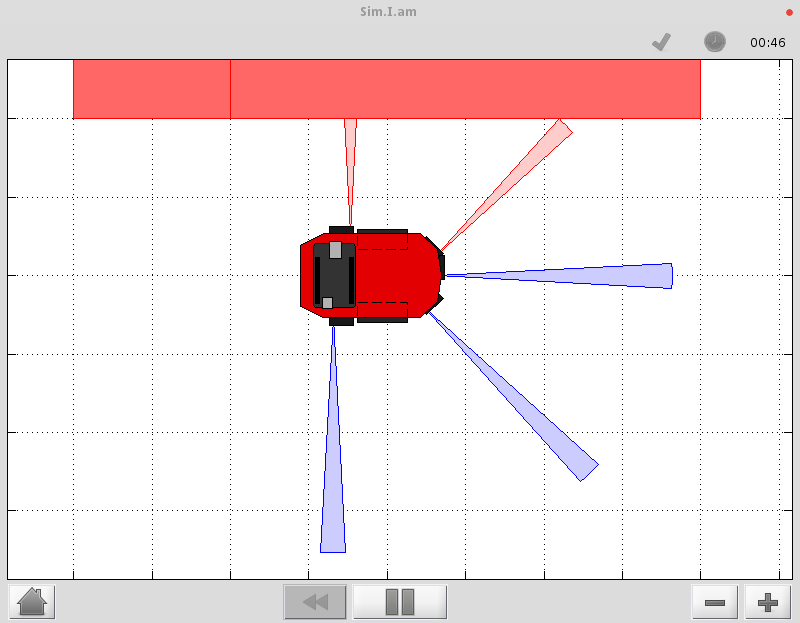
\includegraphics[width=\textwidth]{images/simiam-quickbot.png}
    \caption{Simulated QuickBot}
    \label{fig:simulated-quickbot}
  \end{subfigure}
  \begin{subfigure}{0.45\textwidth}
    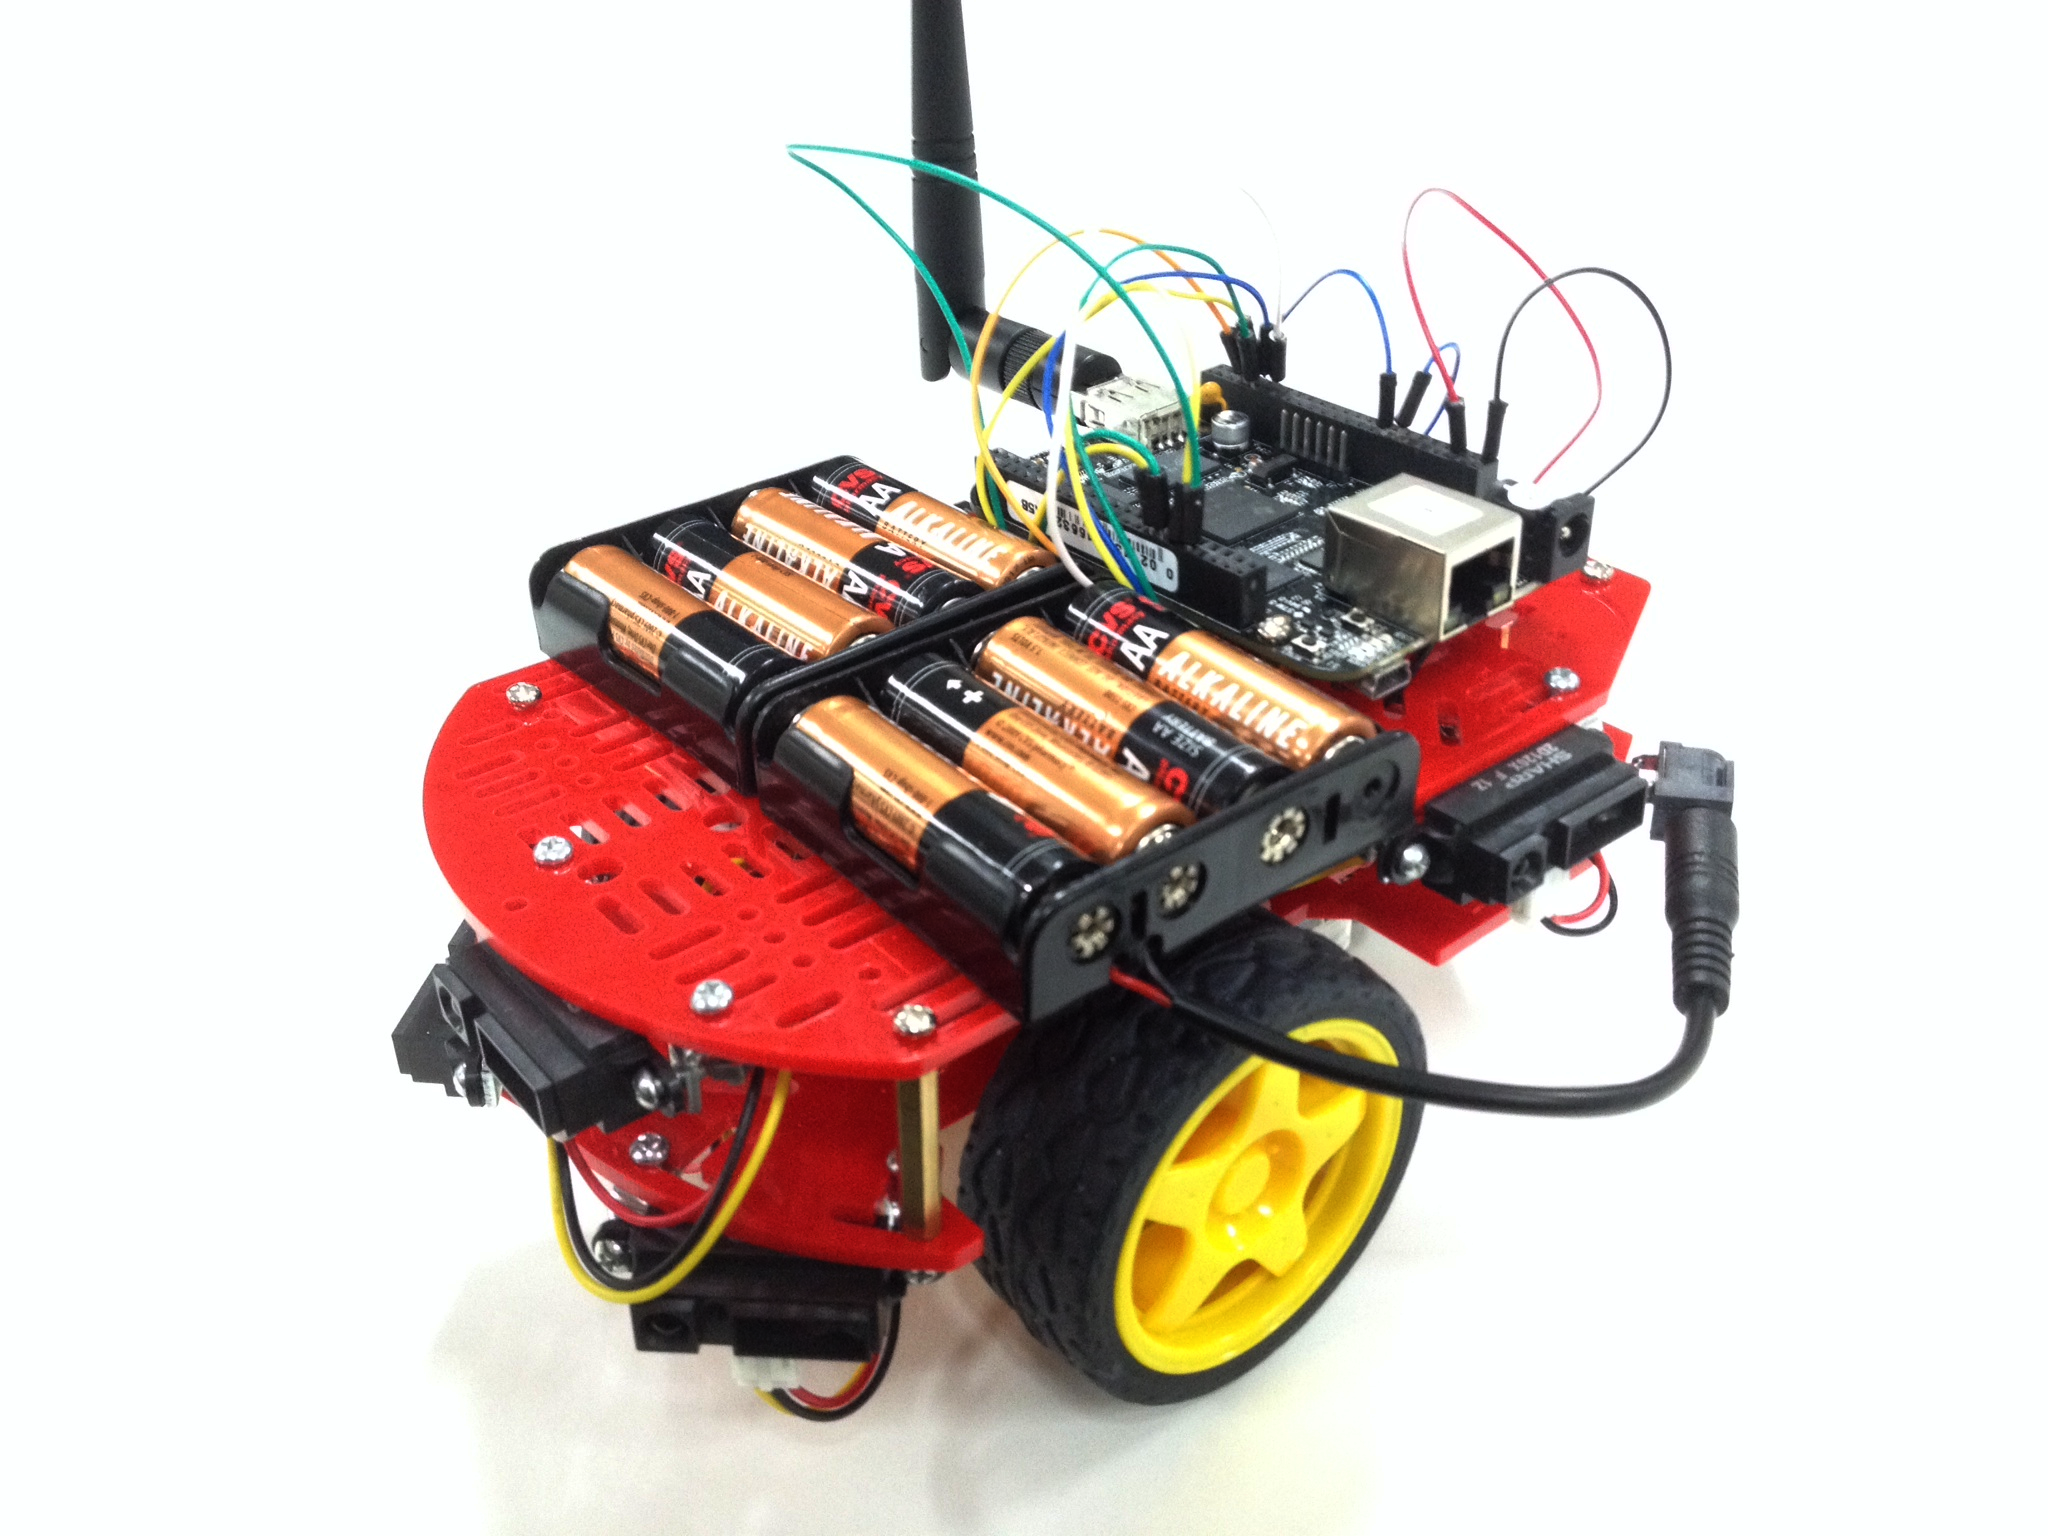
\includegraphics[width=\textwidth]{images/quickbot-red.png}
    \caption{Actual QuickBot}
    \label{fig:actual-quickbot}
  \end{subfigure}
  \caption{The QuickBot mobile robot in and outside of the simulator.}
  \label{fig:quickbot}
\end{figure}

Figure \ref{fig:quickbot} shows the simulated and actual QuickBot mobile robot. The robot simulator recreates the QuickBot as faithfully as possible. For example, the range, output, and field of view of the simulated IR range sensors match the specifications in the datasheet for the actual Sharp GP2D120XJ00F infrared proximity sensors on the QuickBot.

\subsection{IR Range Sensors}\label{irprox}
You will have access to the array of five IR sensors that encompass the QuickBot. The orientation (relative to the body of the QuickBot, as shown in figure \ref{fig:simulated-quickbot}) of IR sensors 1 through 5 is $90^\circ, 45^\circ, 0^\circ$, $-45^\circ, -90^\circ$, respectively. IR range sensors are effective in the range $0.04$ m to $0.3$ m only. However, the IR sensors return raw values in the range of $[0.4,2.75] V$ instead of the measured distances. Figure \ref{fig:ir-volts-meters} demonstrates the function that maps these sensors values to distances. To complicate matters slightly, the BeagleBone Black digitizes the analog output voltage using a voltage divider and a 12-bit, 1.8V analog-to-digital converter (ADC). Figure \ref{fig:ir-adc} is a look-up table to demonstrate the relationship between the ADC output, the analog voltage from the IR proximity sensor, and the approximate distance that corresponds to this voltage.

\begin{figure}[t]
  \centering
  \begin{subfigure}{0.45\textwidth}
    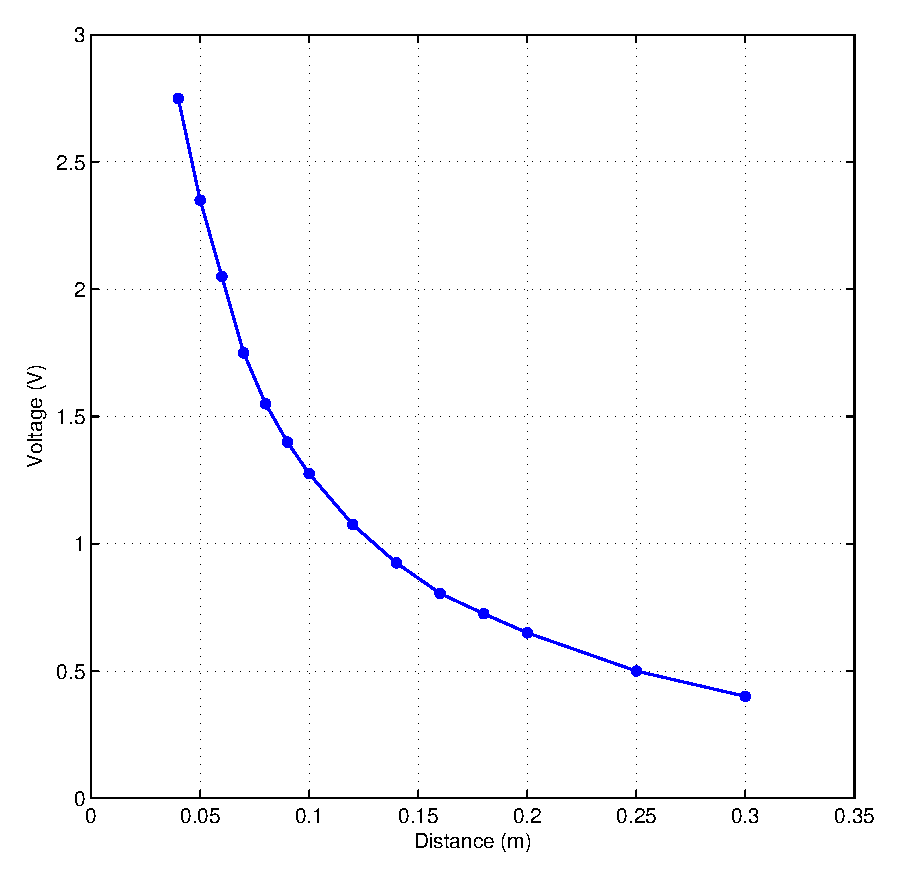
\includegraphics[width=\textwidth]{images/ir-sensor-graph.eps}
    \caption{Analog voltage output when an object is between 0.04m and 0.3m in the IR proximity sensor's field of view.}
    \label{fig:ir-volts-meters}
  \end{subfigure}
  $\qquad$
  \begin{subfigure}{0.45\textwidth}
    \begin{center}
    \begin{tabular}{|p{0.3\textwidth}|p{0.3\textwidth}|p{0.25\textwidth}|}
       \hline
       Distance (m) & Voltage (V) & ADC Out\\
       \hline
       0.04 & 2.750 & 917 \\
       0.05 & 2.350 & 783 \\
       0.06 & 2.050 & 683 \\
       0.07 & 1.750 & 583 \\
       0.08 & 1.550 & 517 \\
       0.09 & 1.400 & 467 \\
       0.10 & 1.275 & 425 \\
       0.12 & 1.075 & 358 \\
       0.14 & 0.925 & 308 \\
       0.16 & 0.805 & 268 \\
       0.18 & 0.725 & 242 \\
       0.20 & 0.650 & 217 \\
       0.25 & 0.500 & 167 \\
       0.30 & 0.400 & 133 \\
       \hline
    \end{tabular}
  \end{center}
    \caption{A look-up table for interpolating a distance (m) from the analog (and digital) output voltages.}
    \label{fig:ir-adc}
  \end{subfigure}
  \caption{A graph and a table illustrating the relationship between the distance of an object within the field of view of an infrared proximity sensor and the analog (and digital) ouptut voltage of the sensor.}
  \label{fig:quickbot}
\end{figure}

Any controller can access the IR array through the \texttt{robot} object that is passed into its \texttt{execute} function. For example,
\begin{verbatim}
  ir_distances = robot.get_ir_distances();
  for i=1:numel(robot.ir_array)
    fprintf('IR #%d has a value of %d', i, robot.ir_array(i).get_range());
    fprintf('or %0.3f meters.\n', ir_distances(i));
  end
\end{verbatim}

It is assumed that the function \texttt{get\_ir\_distances} properly converts from the ADC output to an analog output voltage, and then from the analog output voltage to a distance in meters. The conversion from ADC output to analog output voltage is simply,

\begin{equation*}
  V_{\text{ADC}} = \left\lfloor\frac{1000\cdot V_{\text{analog}}}{3}\right\rceil
\end{equation*}

\textbf{NOTE: For Week 2, the simulator uses a different voltage divider on the ADC; therefore, $V_{\text{ADC}}= V_{\text{analog}}*1000/2$. This has been fixed in subsequent weeks!}

Converting from the the analog output voltage to a distance is a little bit more complicated, because a) the relationships between analog output voltage and distance is not linear, and b) the look-up table provides a coarse sample of points on the curve in Figure \ref{fig:ir-volts-meters}. MATLAB has a \texttt{polyfit} function to fit a curve to the values in the look-up table, and a \texttt{polyval} function to interpolate a point on that fitted curve. The combination of the these two functions can be use to approximate a distance based on the analog output voltage. For more information, see Section \ref{sec:week-2}.

It is important to note that the IR proximity sensor on the actual QuickBot will be influenced by ambient lighting and other sources of interference. For example, under different ambient lighting conditions, the same analog output voltage may correspond to different distances of an object from the IR proximity sensor. This effect of ambient lighting (and other sources of noise) is \textbf{not} modelled in the simulator, but will be apparent on the actual hardware.

\subsection{Differential Wheel Drive}\label{diffdrive}
Since the QuickBot has a differential wheel drive (i.e., is not a unicyle), it has to be controlled by specifying the angular velocities of the right and left wheel $(v_r,v_l)$, instead of the linear and angular velocities of a unicycle $(v,\omega)$. These velocities are computed by a transformation from $(v,\omega)$ to $(v_r,v_\ell)$. Recall that the dynamics of the unicycle are defined as,
\begin{equation}
 \begin{split}
   \dot{x} &= vcos(\theta) \\
   \dot{y} &= vsin(\theta) \\
   \dot{\theta} &= \omega.
 \end{split}
\end{equation}
The dynamics of the differential drive are defined as,
\begin{equation}
 \begin{split}
  \dot{x} &= \frac{R}{2}(v_r+v_\ell)cos(\theta) \\
  \dot{y} &= \frac{R}{2}(v_r+v_\ell)sin(\theta) \\
  \dot{\theta} &= \frac{R}{L}(v_r-v_\ell),
 \end{split}
\end{equation}
where $R$ is the radius of the wheels and $L$ is the distance between the wheels.

The speed of the QuickBot can be set in the following way assuming that the \texttt{uni\_to\_diff} function has been implemented, which transforms $(v,\omega)$ to $(v_r,v_\ell)$:
\begin{verbatim}
 v = 0.15; % m/s
 w = pi/4; % rad/s
 % Transform from v,w to v_r,v_l and set the speed of the robot
 [vel_r, vel_l] = obj.robot.dynamics.uni_to_diff(robot,v,w);
 obj.robot.set_speeds(vel_r, vel_l);
\end{verbatim}

The maximum angular wheel velocity for the QuickBot is approximately 80 RPM or 8.37 rad/s. It is important to note that if the QuickBot is controlled ot move at maximum linear velocity, it is not possible to achieve any angular velocity, because the angular velocity of the wheel will have been maximized. Therefore, there exists a tradeoff between the linear and angular velocity of the QuickBot: \textit{the faster the robot should turn, the slower it has to move forward}.

\subsection{Wheel Encoders}

Each of the wheels is outfitted with a wheel encoder that increments or decrements a tick counter depending on whether the wheel is moving forward or backwards, respectively. Wheel encoders may be used to infer the relative pose of the robot. This inference is called \textbf{odometry}. The relevant information needed for odometry is the radius of the wheel ($32.5$mm), the distance between the wheels ($99.25$mm), and the number of ticks per revolution of the wheel ($16$ ticks/rev). For example,

\begin{verbatim}
 R = robot.wheel_radius; % radius of the wheel
 L = robot.wheel_base_length; % distance between the wheels
 tpr = robot.encoders(1).ticks_per_rev; % ticks per revolution for the right wheel

 fprintf('The right wheel has a tick count of %d\n', robot.encoders(1).state);
 fprintf('The left wheel has a tick count of %d\n', robot.encoders(2).state);
\end{verbatim}

For more information about odometry, see Section \ref{sec:week-2}.

\newpage
\section{Simulator}

Start the simulator with the \texttt{launch} command in MATLAB from the command window. It is important that this command is executed inside the unzipped folder (but not inside any of its subdirectories).

\begin{figure}[h]
  \centering
  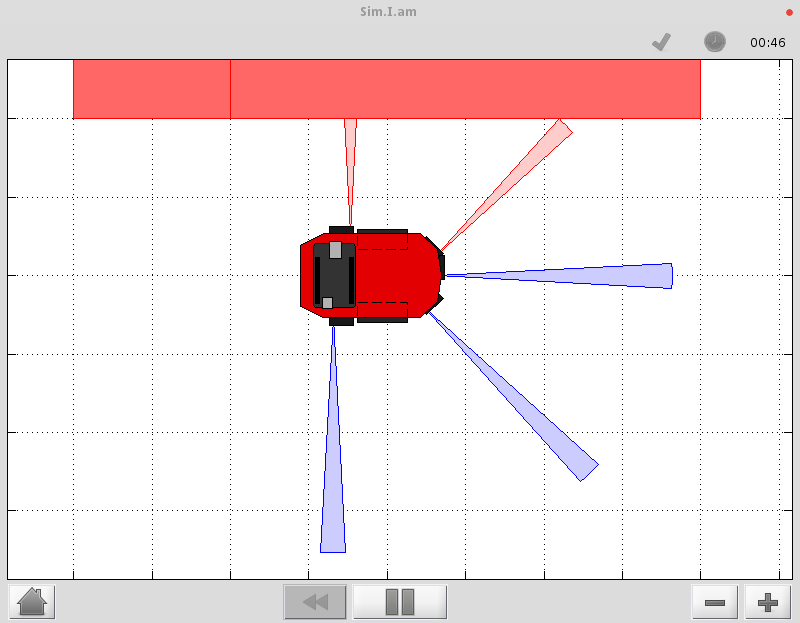
\includegraphics[width=0.45\textwidth]{images/simiam-quickbot.png}
  \label{fig:simulator}
  \caption{\texttt{launch} starts the simulator.}
\end{figure}

Figure \ref{fig:simulator} is a screenshot of the graphical user interface (GUI) of the simulator. The GUI can be controlled by the bottom row of buttons. The first button is the \textit{Home} button and returns you to the home screen. The second button is the \textit{Rewind} button and resets the simulation. The third button is the \textit{Play} button, which can be used to play and pause the simulation. The set of \textit{Zoom} buttons or the mouse scroll wheel allows you to zoom in and out to get a better view of the simulation. Clicking, holding, and moving the mouse allows you to pan around the environment. You can click on a robot to follow it as it moves through the environment.

\newpage
\section{Programming Assignments}

The following sections serve as a tutorial for getting through the simulator portions of the programming exercises. Places where you need to either edit or add code is marked off by a set of comments. For example,

\begin{verbatim}
  %% START CODE BLOCK %%
    [edit or add code here]
  %% END CODE BLOCK %%
\end{verbatim}

To start the simulator with the \texttt{launch} command from the command window, it is important that this command is executed inside the unzipped folder (but not inside any of its subdirectories).

\subsection{Week 1}

This week's exercises will help you learn about MATLAB and robot simulator. \textbf{If you do not already have access to MATLAB, a student license will be made available to registered participants of this course starting Week 2. You can easily put off the optional Week 1 MATLAB assignment until Week 2 without falling behind.} 

\begin{enumerate}
\item Install the GUI Layout Toolbox using the instructions provided in the \emph{Preparing for Programming Assignments} page under \emph{Week 1}. 
\item Familiarize yourself with the simulator by reading this manual and downloading the robot simulator posted on the \textit{Optional Programming Assignment 1: Instructions} section under \emph{Week 1}.
\item Start the simulator by running the \texttt{launch} command from the command window. If the GUI Layout Toolbox has been installed correctly (instructions for this can be found in the \emph{Preparing for Programming Assignments} page under \emph{Week 1}), the home screen should appear. Pressing the Play button will then show a robot which is stationary (it will move once we design controllers for it next week!). 
\end{enumerate}

\end{document}
